\documentclass[12pt,a4paper]{article}
\usepackage[romanian]{babel}
\usepackage[utf8]{inputenc}
\usepackage[T1]{fontenc}
\usepackage{geometry}
\usepackage{graphicx}
\usepackage{hyperref}
\usepackage{float}
\usepackage{amsmath}
\usepackage{listings}

\geometry{margin=2.5cm}

\title{Lucrarea de laborator nr. 3\\
Sistem de monitorizare a duratei apăsărilor unui buton}
\author{Nume Prenume\\Grupa}
\date{\today}

\begin{document}
\begin{titlepage}
\begin{center}
\vspace*{1cm}
{\Large Technical University of Moldova}\\[0.5cm]
{\Large Faculty of Computers, Informatics and Microelectronics}\\[2cm]
{\Huge\bfseries Laboratory Work No. 2.1}\\[1cm]
{\Large\bfseries Embedded Systems:\\
Button Duration Monitor with Visual Signaling\\
and Periodic Reporting}\\[3.5cm]
\begin{flushright}
\begin{tabular}{ll}
\textbf{Elaborated:} & \\
std. gr. FAF-231 & Burduja Adrian \\[1cm]
\textbf{Verified:} & \\
asist. univ. & Alexei Martîniuc \\ & \\
\end{tabular}
\end{flushright}
\vfill
{\Large Chișinău -- 2026}
\end{center}
\end{titlepage}
\tableofcontents
\newpage

%-------------------------------------------------
\section{Task Analysis and Technological Context}

\subsection{Domain Analysis and Technological Context}
Multitasking embedded systems are widely used in monitoring applications,
human--machine interfaces, and real-time control. Monitoring the duration of an input action
(button press) is relevant in industrial systems, consumer electronics, and educational systems,
where the same physical interface may have different meanings depending on the interaction duration.

This work addresses this problem by implementing a multitasking system that clearly separates
data acquisition, statistical processing, and user reporting.

\subsection{External Resources and Bibliographic References}
The following types of resources were used:
\begin{itemize}
    \item documentation of the used microcontroller;
    \item documentation of the real-time operating system (RTOS);
    \item official examples regarding task management and timing;
    \item educational materials provided within the course.
    	\item Chat gpt for writting the structure of the report and some of the text
	\item Deepseek for helping with code
\end{itemize}


\subsection{Analysis of Components and Used Resources}
The system uses:
\begin{itemize}
    \item a microcontroller with multitasking support;
    \item a digital input push button;
    \item three LEDs (green, red, yellow);
    \item STDIO interface for reporting;
    \item software resources: tasks, logically protected global variables, and timers.
\end{itemize}

%-------------------------------------------------
\section{Definition of Technical Requirements and Test Scenarios}

\subsection{Application Objectives}
The main objective is the design and implementation of a multitasking application that:
\begin{itemize}
    \item detects button presses;
    \item measures their duration;
    \item visually signals the press type;
    \item collects statistics;
    \item periodically reports results.
\end{itemize}


\subsection{Functional and Non-Functional Requirements}

\textbf{Functional requirements:}
\begin{itemize}
    \item detection of press/release transitions;
    \item duration measurement in milliseconds;
    \item classification of presses into short and long;
    \item visual signaling using LEDs;
    \item periodic reporting via STDIO;
    \item statistics reset after reporting.
\end{itemize}

\textbf{Non-functional requirements:}
\begin{itemize}
    \item clear separation of responsibilities across tasks;
    \item temporal determinism;
    \item code readability and modularity;
    \item low resource consumption.
\end{itemize}

\subsection{Test Scenarios and Validation Criteria}
\begin{itemize}
    \item short press ($<500\,ms$) – green LED active;
    \item long press ($\geq500\,ms$) – red LED active;
    \item verification of the number of yellow LED blinks;
    \item correct reporting every 10 seconds;
    \item correct reset of statistics after reporting.
\end{itemize}

%-------------------------------------------------
\section{Architectural Design and Behavioral Modeling}

\subsection{System Components}
\begin{itemize}
    \item Detection Task – monitors the button and measures duration;
    \item Statistics Task – updates counters and yellow LED signaling;
    \item Reporting Task – sends data via STDIO;
    \item Hardware I/O – button and LEDs;
    \item STDIO Interface.
\end{itemize}

\newpage
\subsection{Structural Diagram}
\begin{figure}[!ht]
    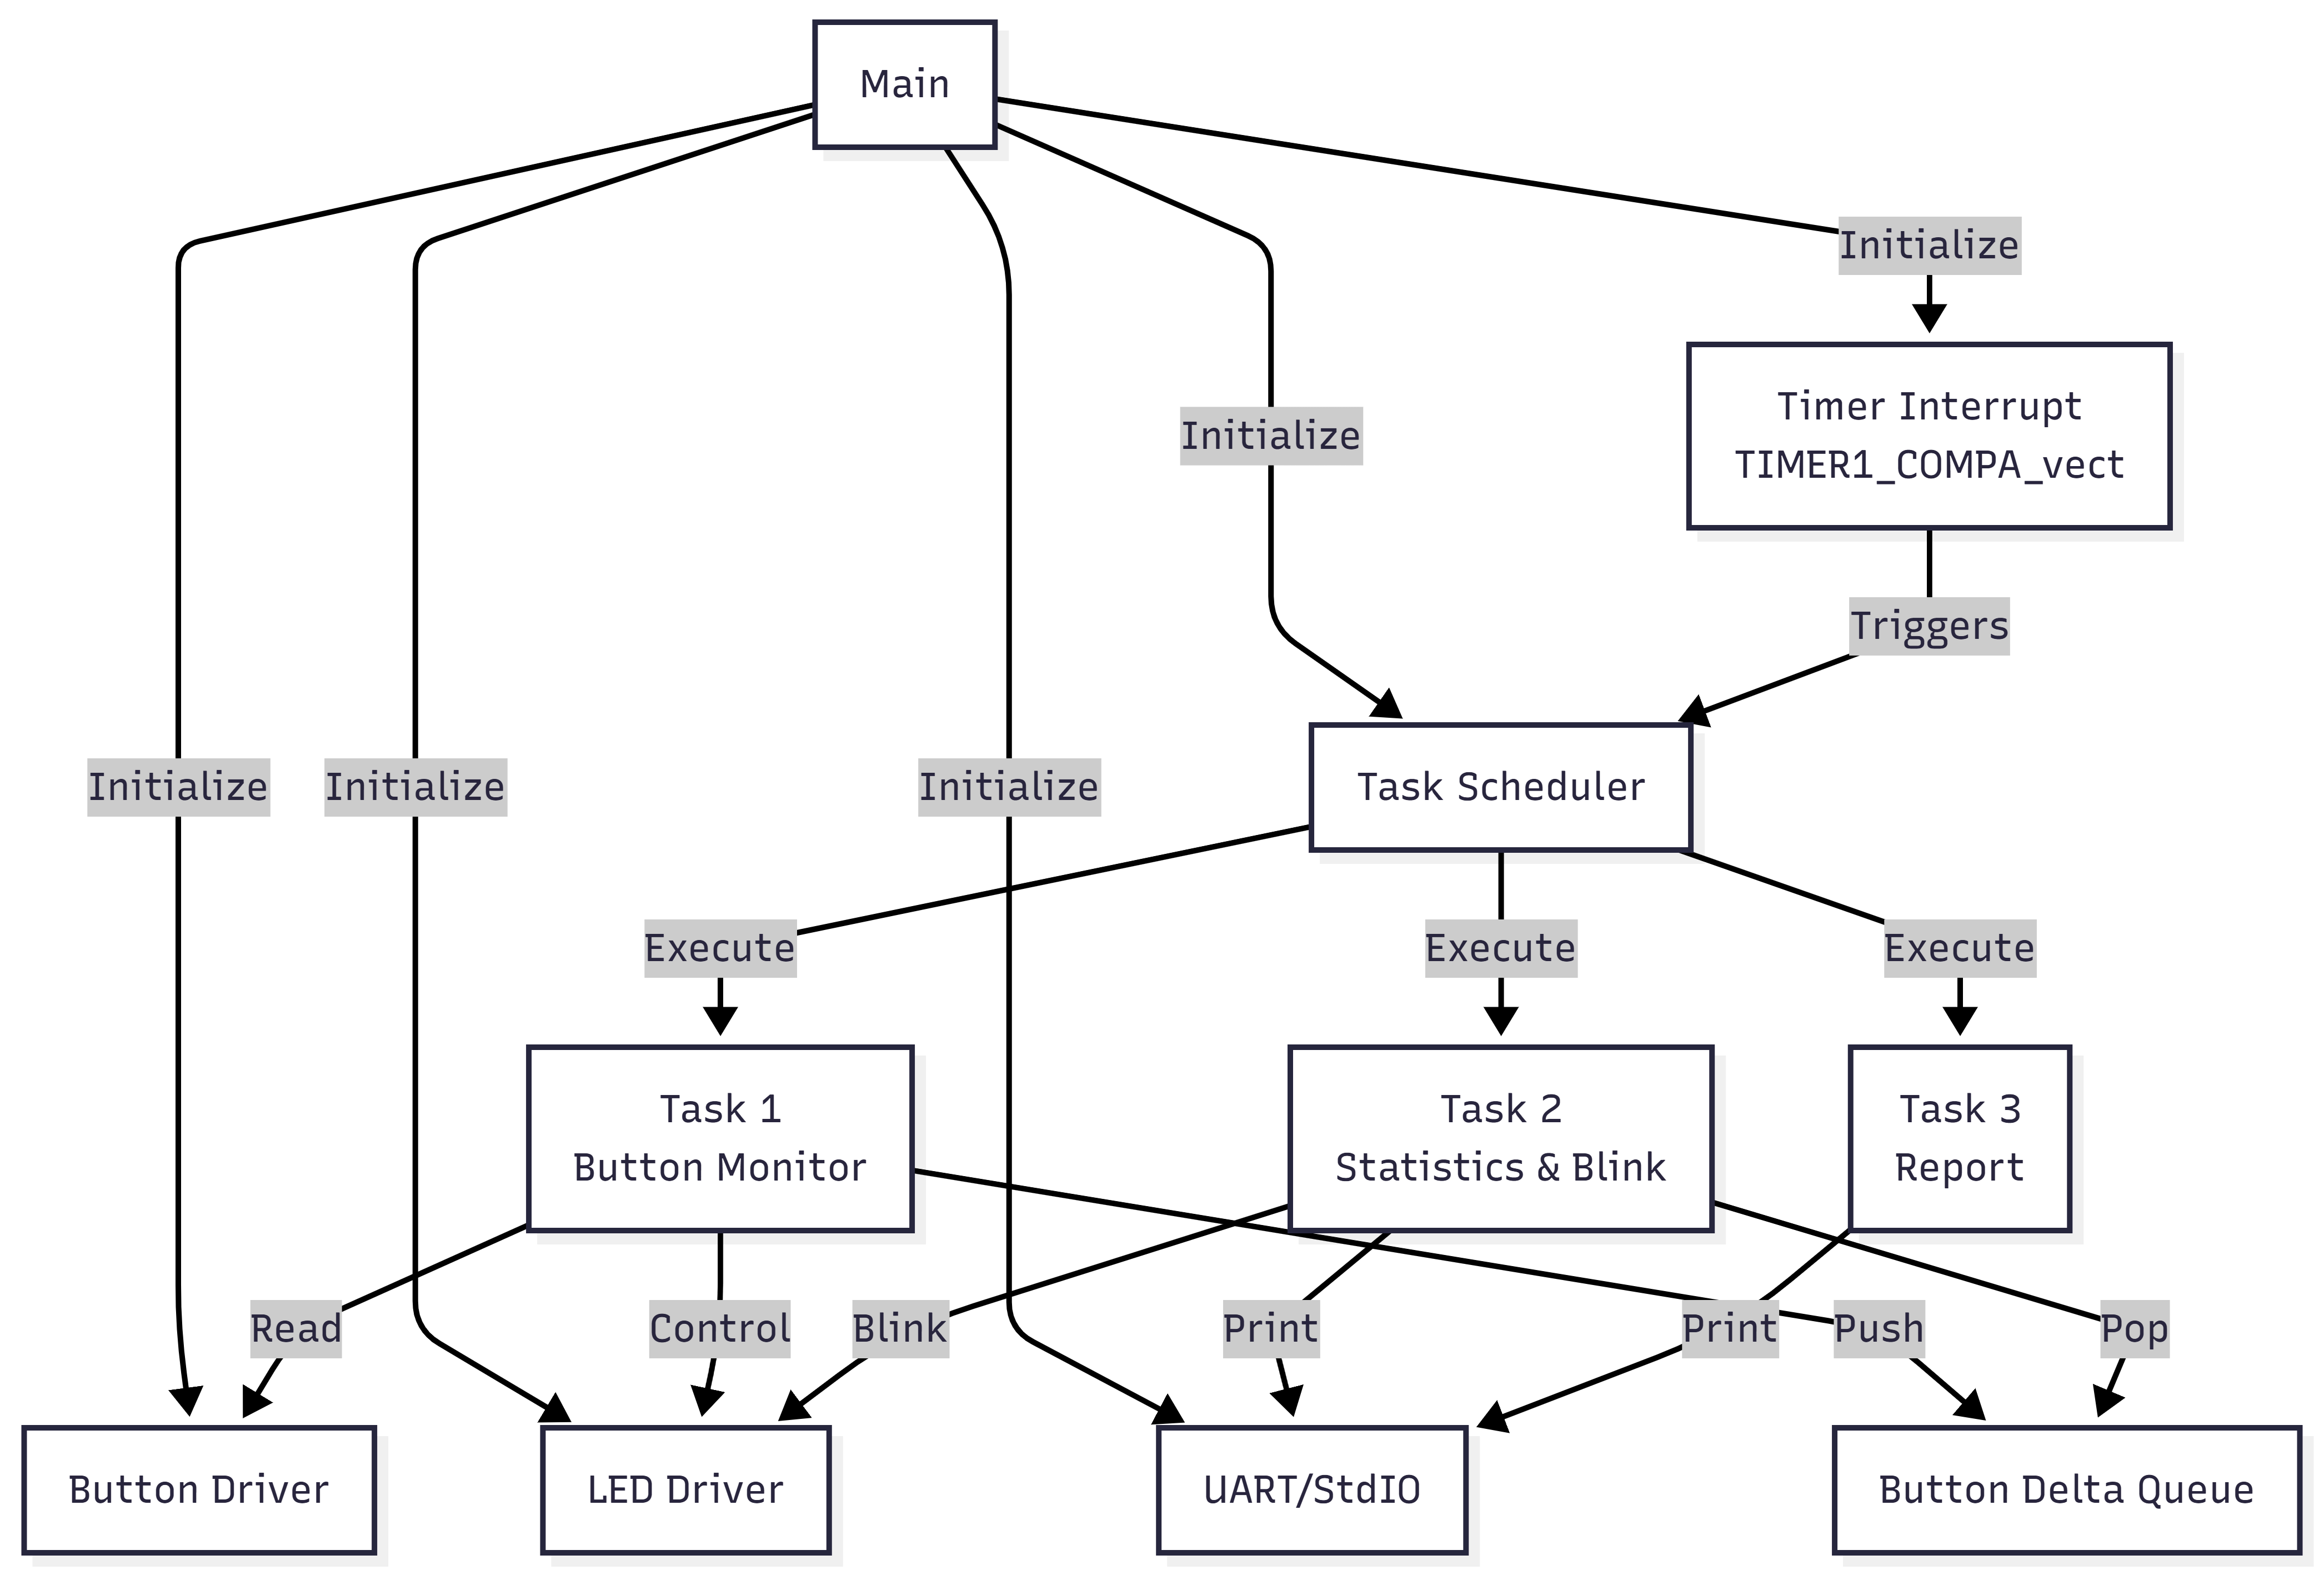
\includegraphics[width=0.8\textwidth]{img/structure.png}
    \caption{Architectural sketch}
\end{figure}

\subsection{HW--SW Layered Architecture}
The application is organized into the following layers:
\begin{itemize}
    \item hardware layer (button, LEDs);
    \item HAL layer (GPIO drivers, timing);
    \item RTOS layer (tasks, scheduler);
    \item application layer (logic and statistics).
\end{itemize}

\newpage
\subsection{Behavioral Diagrams}
\begin{figure}[!ht]
    \includegraphics[width=0.8\textwidth]{img/sequence.png}
    \caption{Behavioral sketch}
\end{figure}

%-------------------------------------------------
\newpage
\section{Electrical Schematic Design and Simulation}

\subsection{Electrical Schematic}
\begin{figure}[!ht]
    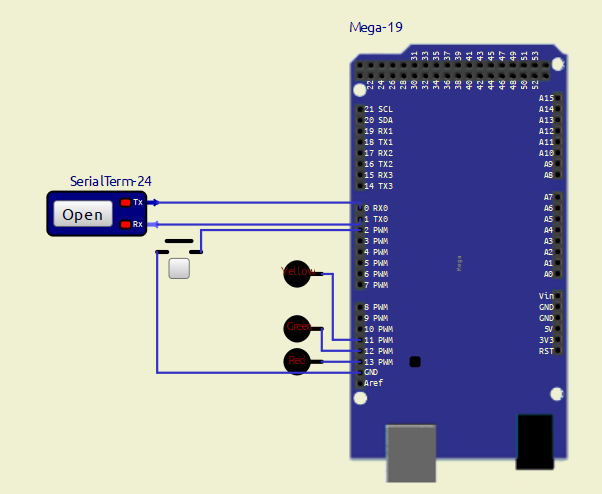
\includegraphics[width=0.8\textwidth]{img/sim.PNG}
    \caption{Behavioral sketch}
\end{figure}

\subsection{Connections and Component Sizing}
The button is connected to a digital input pin using a pull-up resistor, and the LEDs
are connected through appropriate current-limiting resistors.

\subsection{Simulation}
The application was simulated in a virtual environment to validate logic and timing behavior. The simulator is called SimulIDE.

\subsection{Execution on Real Hardware}
Results of running the application(terminal output):
\begin{lstlisting}
just pushed, 1
Pushed delta 150
just pushed, 1
Pushed delta 1849
Numarul de apasari: 2
Numarul de apasari scurte: 1
Numarul de apasari lungi:  1
Durata medie a apasarilor: 999
\end{lstlisting}

%-------------------------------------------------
\section{Modular Software Implementation}

\subsection{Project Structure}
\begin{lstlisting}
build\
baremetal.ino
build.bat
button_driver.c
button_driver.h
inter.c
inter.h
leds_driver.c
leds_driver.h
main.c
queue.c
queue.h
stdio_layer.c
stdio_layer.h
task_procs.c
task_procs.h
\end{lstlisting}



\subsection{HW--SW Interface}
Dedicated functions are used for GPIO access and timing, separated from the application logic.

\subsection{Behavior Implementation}
Each task implements a clearly defined role, according to the initial design.

\subsection{Comments and Documentation}
The code is commented to highlight the logic and design decisions.

%-------------------------------------------------
\section{Simulation, Testing, and Validation}

\subsection{Testing}
Tests were performed according to the previously defined scenarios.

\subsection{Results and Observations}
The obtained results confirm the correct operation of the application.

\subsection{Optimizations}
Optimizations related to timing and task organization were identified.

%-------------------------------------------------
\section{Conclusions}

The developed application demonstrates the effective use of multitasking in an embedded system.
Separating functionality across tasks improves clarity, scalability, and system reliability.
The solution can be easily extended for more complex applications.

\newpage
\section{Annex}

\subsection{ button\_driver.c }
\begin{lstlisting}
#include "button_driver.h"
#include <Arduino.h>

#define BUTT_PIN 2

void init_button()  { pinMode(BUTT_PIN, INPUT_PULLUP); }
bool is_button_up() { return digitalRead(BUTT_PIN);    }
\end{lstlisting}

\subsection{button\_driver.h}
\begin{lstlisting}
#pragma once

#include <stdbool.h>
void init_button();

bool is_button_up();
\end{lstlisting}

\subsection{inter.c}
\begin{lstlisting}
#include "inter.h"
#include <avr/io.h>
#include <avr/interrupt.h>

void init_clock(){
	// Disable interrupts while we configure Timer1
	// Disable interrupts during setup
	cli();

	// Reset Timer1 registers to a known state
	TCCR1A = 0;
	TCCR1B = 0;
	TCNT1 = 0;

	// Set compare match register for a 1 Hz interrupt (16MHz/64/25000 = 10Hz, use 25000 for 0.5Hz? Let's use 15624 for 1Hz)
	// Formula: OCR1A = (16,000,000 / (prescaler * desired freq)) - 1
	// For 1 Hz: (16e6 / (256 * 1)) - 1 = 62499 (too high for 16-bit)
	// For 2 Hz with /256: (16e6 / (256 * 2)) - 1 = 31249
	// For 1 Hz with /1024: (16e6 / (1024 * 1)) - 1 = 15624
	OCR1A = 15624/(2<<10); // Interrupt roughly once per second

	// Turn on CTC mode (WGM12 = 1)
	TCCR1B |= (1 << WGM12);

	// Set prescaler to 1024 (CS12 = 1, CS10 = 1)
	TCCR1B |= (1 << CS12) | (1 << CS10);

	// Enable timer compare interrupt
	TIMSK1 |= (1 << OCIE1A);

	// Re-enable global interrupts
	sei();
}
\end{lstlisting}

\subsection{inter.h}
\begin{lstlisting}
#pragma once
#include <Arduino.h>

void init_clock();
\end{lstlisting}

\subsection{leds\_driver.c}
\begin{lstlisting}
#include "leds_driver.h"
#include <Arduino.h>

// Register controll
#define RED_LED_PIN 13
#define GREEN_LED_PIN 12
#define YL_LED_PIN 11

void init_leds(){
	pinMode(RED_LED_PIN,   OUTPUT);
	pinMode(GREEN_LED_PIN, OUTPUT);
	pinMode(YL_LED_PIN,    OUTPUT);

	yl_led_turn_off();
	red_led_turn_off();
	green_led_turn_off();
}

void red_led_turn_on()  { digitalWrite(RED_LED_PIN,HIGH); }
void red_led_turn_off() { digitalWrite(RED_LED_PIN, LOW); }

void green_led_turn_on()  { digitalWrite(GREEN_LED_PIN,HIGH); }
void green_led_turn_off() { digitalWrite(GREEN_LED_PIN, LOW); }

void yl_led_turn_on()  { digitalWrite(YL_LED_PIN,HIGH); }
void yl_led_turn_off() { digitalWrite(YL_LED_PIN, LOW); }

#define BLINK_LEN 100

int blink_counter = 0;
int blink = LOW;
bool executing;
void yl_exec_blink(){
	if (blink_counter == 0) { return; }

	int now = millis();
	if(now % 100 == 0){
		blink = blink? LOW:HIGH;
		blink_counter -=1;
	}
	
	digitalWrite(YL_LED_PIN, blink );
}

void yl_setup_blink(int n){
	blink_counter = n*2;
}
\end{lstlisting}

\subsection{leds\_driver.h}
\begin{lstlisting}
#pragma once

#include <stdbool.h>
void init_leds();
void init_button();

void red_led_turn_on();
void red_led_turn_off();
void green_led_turn_on();
void green_led_turn_off();
void yl_led_turn_on();
void yl_led_turn_off();

void yl_exec_blink();
void yl_setup_blink(int);

bool is_button_up();
\end{lstlisting}

\subsection{main.c}
\begin{lstlisting}
// baremetal version
#include <Arduino.h>
#include <stdbool.h>
#include <stdio.h>
#include "stdio_layer.h"
#include "task_procs.h"
#include "button_driver.h"
#include "leds_driver.h"
#include "inter.h"


task_t tasks[3];

int main(void){
	init();
	init_button();
	init_leds();
	init_stdout();
	init_tasks(tasks);

	for (int i=0; i<TASK_N;++i) {
		printf("%d context count  %d\n",i,tasks[i].context.cnt);
		printf("%d context offset %d\n",i,tasks[i].context.offset);
		printf("%d context rec    %d\n",i,tasks[i].context.rec);
	
	}

	init_clock();
	
	for(;;){
	}
	return 0;
}

ISR(TIMER1_COMPA_vect){ // main loop
	for (int i=0; i<TASK_N;++i) {
		context_t ctx = tasks[i].context;
		context_proc* proc = tasks[i].proc;
		if (ctx.cnt > 0) { 
			ctx.cnt -=1; 
		} else {
			ctx.cnt = ctx.offset;
			proc();
		}
		tasks[i].context = ctx;
	}
}
\end{lstlisting}

\subsection{queue.c}
\begin{lstlisting}
#include "queue.h"

void push(Button_deltas *stack, unsigned long in_item) {
	stack->els[stack->idx] = in_item;       
	stack->idx = (stack->idx+1) % MAX_STACK;
}

unsigned long pop(Button_deltas *stack){
	stack->idx = (stack->idx+MAX_STACK - 1) % MAX_STACK;
	return stack->els[stack->idx];                  
}
\end{lstlisting}

\subsection{queue.h}
\begin{lstlisting}
#pragma once

#define MAX_STACK 255

typedef struct {
	unsigned long els[MAX_STACK]; 
	int  idx;
}Button_deltas;

void push(Button_deltas *stack, unsigned long in_item);
unsigned long pop(Button_deltas *stack);
\end{lstlisting}

\subsection{stdio\_layer.c}
\begin{lstlisting}
#include "stdio_layer.h"
#include <stdio.h>
#include <Arduino.h>
// Code generated by claude
// start

int uart_putchar(char c, FILE *stream) {
	if (c == '\n') { uart_putchar('\r', stream); }
	while(!(UCSR0A & (1 << UDRE0)));
	UDR0 = c;
	return 0;
}

int uart_getchar(FILE *stream) {
	while(!(UCSR0A & (1 << RXC0)));
	return UDR0;
}

FILE uart_str = FDEV_SETUP_STREAM(uart_putchar, uart_getchar, _FDEV_SETUP_RW);

void uart_init(unsigned long baud){
	unsigned int ubrr = F_CPU/16/baud - 1;
	UBRR0H = (ubrr >> 8);
	UBRR0L = ubrr;
	UCSR0B = (1 << TXEN0) | (1 << RXEN0);
	UCSR0C = (3 << UCSZ00);

	stdout = &uart_str;
	stdin = &uart_str;
}

// end

void init_stdout(){ uart_init(9600); }

// IO
#define BUFFER_SIZE 255
char _buffer[BUFFER_SIZE+1];
char* buffer(){return _buffer;}

int _bufflen = 0;
int bufflen(){return _bufflen;}

void read_input(){
	fgets(_buffer, BUFFER_SIZE, stdin);
	_bufflen = strlen(_buffer);
}

void print_input(){ printf("%s", _buffer); }
\end{lstlisting}

\subsection{stdio\_layer.h}
\begin{lstlisting}
#pragma once
#include <stdio.h>

// forward decl for Arduino.h function
int strncmp(const char *, const char *, unsigned int);

void uart_init(unsigned long baud);
int uart_putchar(char c, FILE *stream);
int uart_getchar(FILE *stream);

char* buffer();
int bufflen();

void init_stdout();

void read_input();
void print_input();
\end{lstlisting}

\subsection{task\_procs.c}
\begin{lstlisting}
#include "task_procs.h"

#include "button_driver.h"
#include "leds_driver.h"
#include "queue.h"
#include <stdbool.h>
#include <stdio.h>
#include "Arduino.h"

#define TASK1_OFFSET 0
#define TASK2_OFFSET 1
#define TASK3_OFFSET 255

#define TASK1_REC 0
#define TASK2_REC 1
#define TASK3_REC 255

void init_tasks(task_t *tasks){ 
	tasks[0] = (task_t){
		.context = (context_t) {TASK1_OFFSET,TASK1_OFFSET,TASK1_REC},
		.proc = task1_proc,
	}; 
	tasks[1] = (task_t){
		.context = {TASK2_OFFSET,TASK2_OFFSET,TASK2_REC},
		.proc =task2_proc,	
	};
	tasks[2] = (task_t){
		.context = {TASK3_OFFSET,TASK3_OFFSET,TASK3_REC},
		.proc = task3_proc,
	};
}

// button state global vars
bool button_prev_state = HIGH; 
bool button_state = HIGH;
unsigned long button_timestamp; 
int button_duration;

// stack(unsigned long) Button_deltas;
Button_deltas button_deltas;

// manage press intervals
void task1_proc(void){
	bool button_state = is_button_up();

	// handle state of button changed
	if(button_state != button_prev_state) {

		unsigned long now = millis();

		// if the button was released 
		if (button_state) {
			button_duration = now - button_timestamp;
			push(&button_deltas, button_duration);
			printf("just pushed, %d\n",button_deltas.idx);

			if (button_duration < 500){
				// short hold
				green_led_turn_on();
				red_led_turn_off();
			} else {
				// long hold
				red_led_turn_on();
				green_led_turn_off();
			}

		} else {
			// if button was pressed
			button_timestamp = now;
		}
		button_prev_state = button_state;
	}
	// else, nothing happens
}

#define LONG_PRESS 500
int presses,sum_shorts,sum_longs,n_shorts,n_longs;
// manage press statistics
void task2_proc(void){
	yl_exec_blink();	
	
	// button was pressed and released, ie a delta was pushed onto the stack
	if (button_deltas.idx > 0) {
		unsigned long delta = pop(&button_deltas);
		printf("Pushed delta %lu\n",delta);
			
		presses +=1;
		if (delta < LONG_PRESS) {
			sum_shorts = sum_shorts + delta;
			n_shorts += 1;
			yl_setup_blink(5);
		} else {
			sum_longs = sum_longs + delta;
			n_longs += 1;
			yl_setup_blink(10);
		}
	}
}


#define REPORT_INTERVAL 10
unsigned long report_timestamp;

void task3_proc(void){

	unsigned long now = millis();
	if((now - report_timestamp)/1000 < REPORT_INTERVAL ) return;

	report_timestamp = now;

	unsigned long averege_holds = sum_longs + sum_shorts;
	printf("Durata medie a apasarilor: %lu\n",averege_holds);
		
	
	if (n_longs+n_shorts > 0) {
		averege_holds = averege_holds / (n_longs+n_shorts);
	}


	printf(
		"Numarul de apasari: %d\n"
		"Numarul de apasari scurte: %d\n"
		"Numarul de apasari lungi:  %d\n"
		"Durata medie a apasarilor: %lu\n",
		n_shorts+n_longs,
		n_shorts,
		n_longs,
		averege_holds
	);

	// reset
	n_shorts =0;
	n_longs = 0;
	sum_shorts = 0;
	sum_longs  = 0;
}
\end{lstlisting}

\subsection{task\_procs.h}
\begin{lstlisting}
#pragma  once
#include <stdio.h>

typedef struct {
	uint8_t cnt;
	uint8_t offset;
	uint8_t rec;
} context_t;

typedef void context_proc(void);

typedef struct{
	context_t context;
	context_proc* proc;
} task_t ;
enum {
	TASK_1 = 0,
	TASK_2,
	TASK_3,
	TASK_N
};


void task1_proc(void);
void task2_proc(void);
void task3_proc(void);

void init_tasks(task_t *tasks);
\end{lstlisting}


\end{document}